\subsection{Frontend Implementering}
\label{sec:Frontend Implementering}
Det endelige design af vinderne(vinduerne?) følger tæt det oprindelige mockup design. Der benyttes MVVM (Model, View and View Model) designpatterns.  Det har undervejs i implementeringen vist sig et behov for væsentlig flere menuer end først antaget, og disse er implementeret efter samme overordnede design, som resten af systemet, så derved følges stilen og følelsen af spillet.\\
Det endelige design har følgende views:
Login, Register, Main, Settings, Ingame, Load, Save, Inventory, Character, Victory, Defeat, Room og Combat.\\
Til at skifte views uden at oprette et nyt vindue bruges et mediator design, hvor hver knap som skifter view giver en besked til mediatoren. Dette virker fordi alle views er oprettet som WPF user controlls, og ikke views, hvilket tillader at et main view kan skifte mellem viewmodels, derved skifter vil alt indhold på vinduet, men uden at selve rammen skifter. Dette resulterer i et mere flydende User Interface for brugeren og derved en alt i alt bedre oplevelse. \cite{Mediator}\\
Et eksempel på hvordan mediatoren kaldes ved et tryk på en knap kan ses i følgende kode eksempel:

\begin{lstlisting}[language=c]
private DelegateCommand _loadGame;
    
public DelegateCommand LoadGame => _loadGame ?? (
	_loadGame = new DelegateCommand(
	ExecuteLoadCommand, CanExecuteLoadCommand));

async void ExecuteLoadCommand()
{
    await GameController.Instance.LoadGame(SelectedSave.ID);
    Mediator.Notify("GameStart", "");
}

bool CanExecuteLoadCommand()
{
    return SelectedSave != null;
}

void LoadCommand()
{
    LoadGame.RaiseCanExecuteChanged();
}
\end{lstlisting}

\noindent Der er implementeret at nogle af spillets funktioner kan tilgås via key-bindings, hvilket har nødsaget et brud på MVVM-designet. Når mediatoren skifter mellem views bilver fokus ikke sat til indholdet af det nye view, og keybindings virker derfor ikke. For at løse dette sættes top-elementet på den nye side som fokus. Dette kan dog ikke gøres i MVVM, så her er det pattern brudt, da det er nødvendigt at gå ind i code-behind filen for at sætte fokus.

\noindent De følgende afsnit viser et udvalg af view, samt en beskrivelse af hvordan de afviger fra det oprindelige design og en beskrivelse af interesante programerings-tekniske beslutninger.

\subsubsection{Login view}
Den overordnede struktur af login (\autoref{fig:Design-FE-impl-login}) og register menuerne følger meget tæt det oprindelige design. Alle elementer er blevet stiliseret så de matcher det ønskede look. Dette er gjort ved brug af globale resourses og styles i app.xaml filen(\textbf{INDSÆT REFERENCE TIL HVOR FILEN KAN FINDES HER}). Dette gør det nemt at oprette nye views og ændre udseende af hele spillet. Selve login håndteres af backenden som kaldes af login og register knapperne via command bindings.

\begin{figure}[H]
\centering
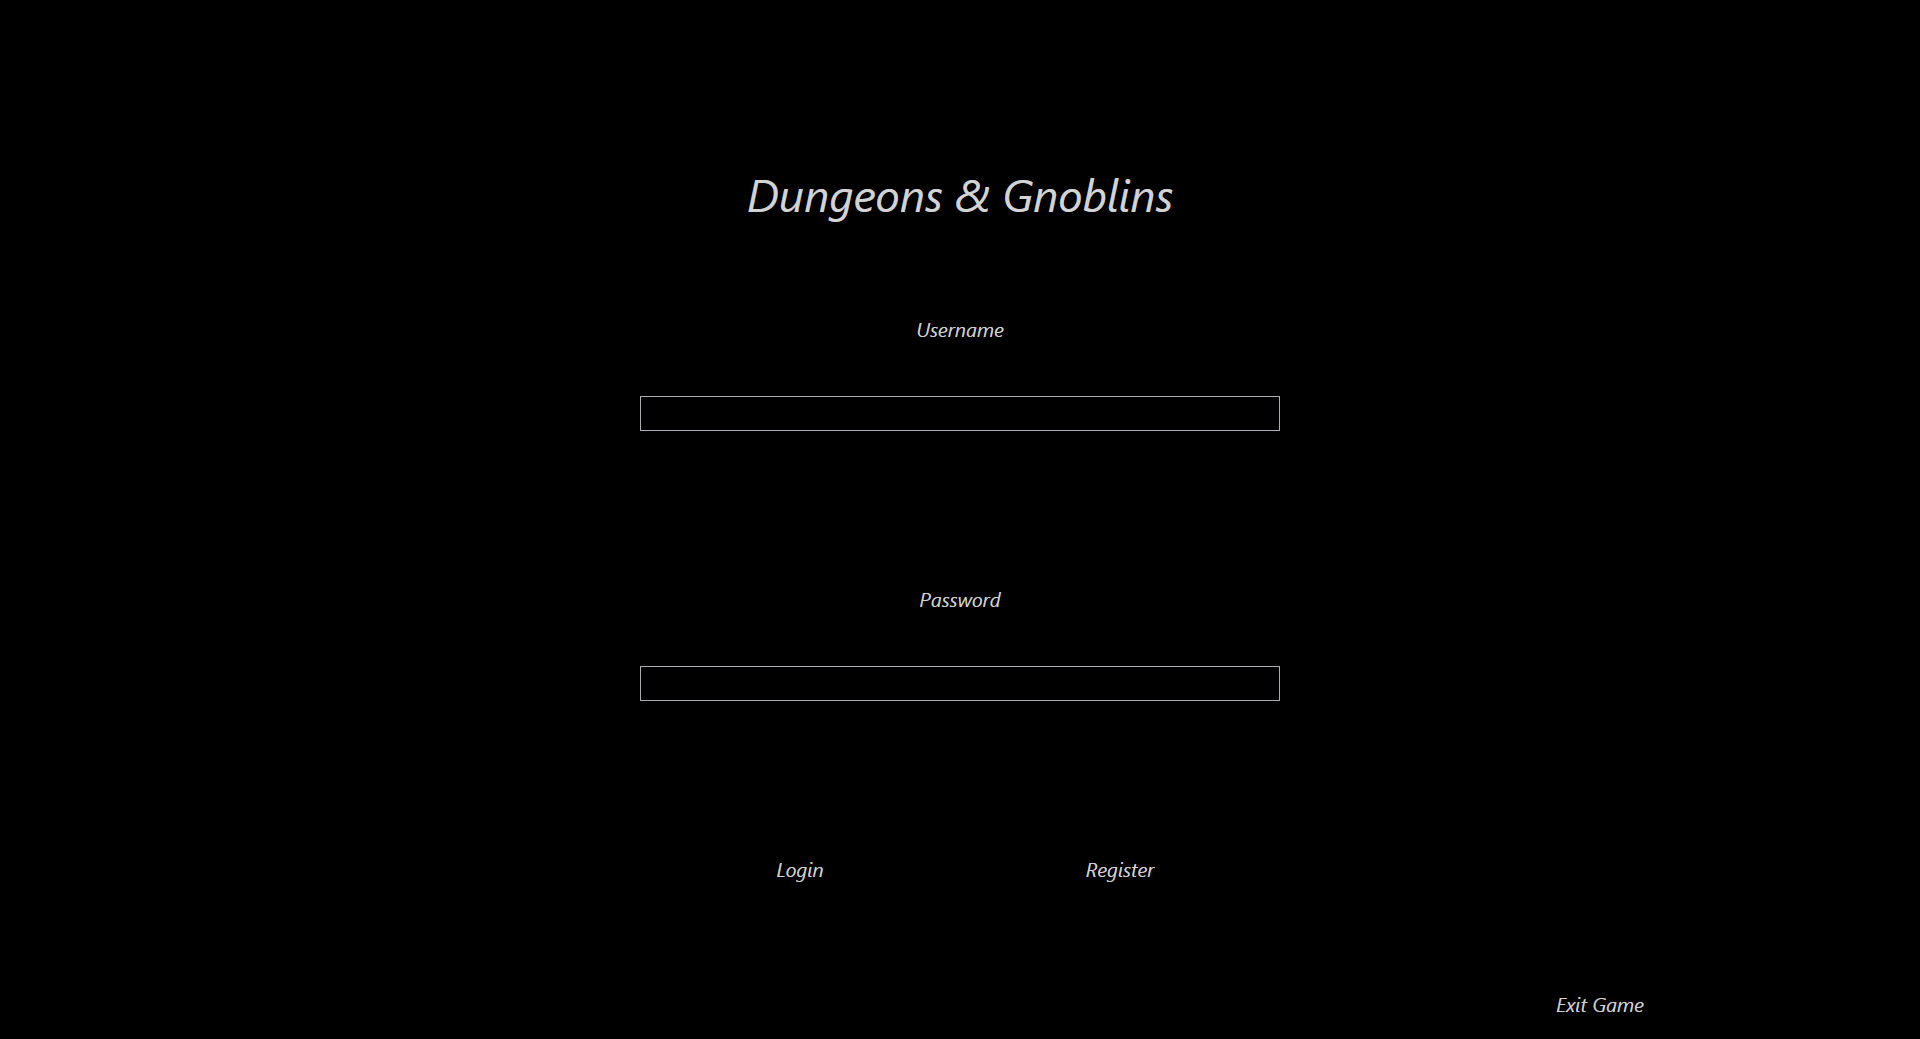
\includegraphics[width = \textwidth]{02-Body/Images/login_final.PNG}
\caption{Endelig login skærm. Brugenavn og kodeord kan indtastes i de to felter. Register knappen fører til et nyt view, hvor man kan oprætte en bruger, mens login knappen fører spilleren til main menu, hvis deres login er korrekt.}
\label{fig:Design-FE-impl-login}
\end{figure}

\subsubsection{Room View}

Visuelt er room view (\autoref{fig:Design-FE-impl-room}) ikke ændret betydeligt fra det oprindelige design. Der er ændret lidt på placering og antal af knapper så det passer til antallet af interaktioner tilgængelig til brugeren. Kortet er lavet så det  opdateres når spilleren går ind i et nyt rum, ved at ændre på synligheden af elementerne i kortet. Det er yderligere sat op så det kan skaleres til de skærmopløsninger som understøtes.\\
Ved at trykke på interact knappen kan spilleren flytte et valgt 'item' fra listen nederst til venstre over i sit inventory (et seperat view), som kan tilgås ved at trykke på Inventory knappen.\\
Alt tekst er vist med data binding.

\begin{figure}[H]
\centering
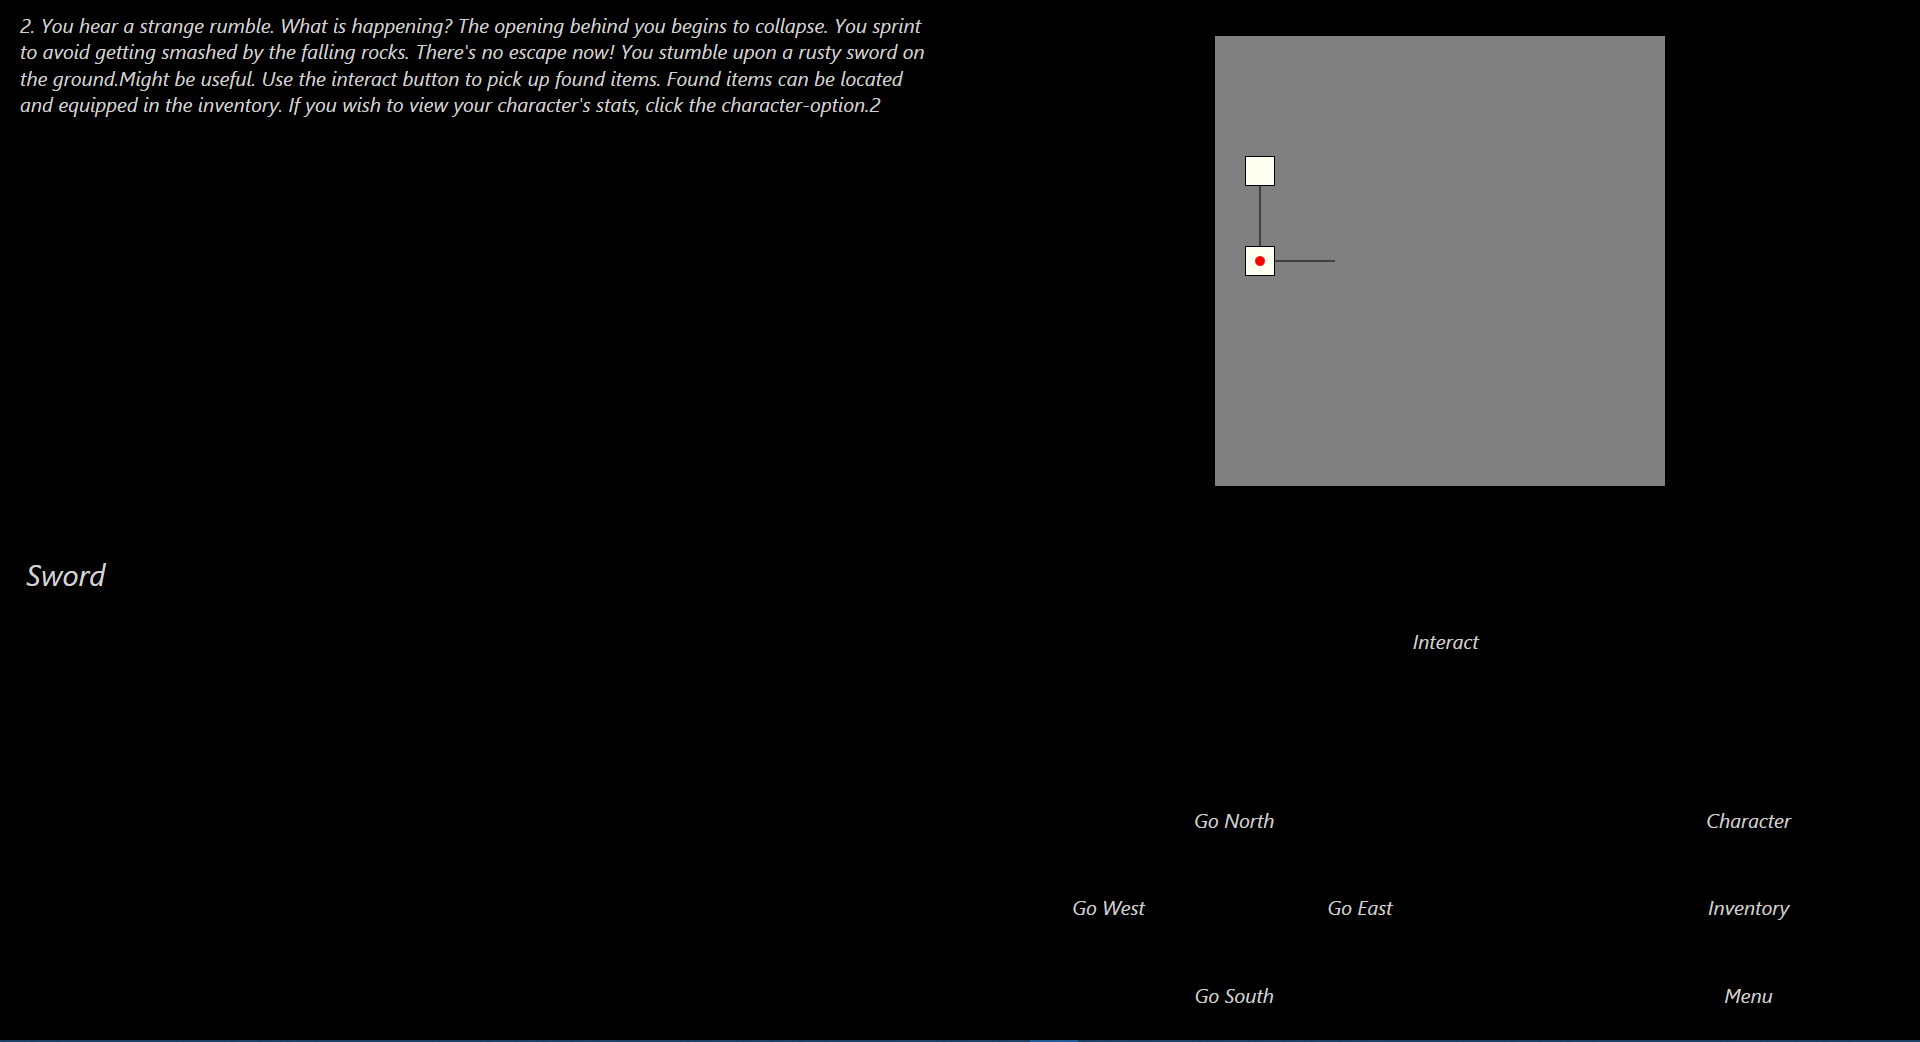
\includegraphics[width = \textwidth]{02-Body/Images/room_final.PNG}
\caption{Endeligt udseende af room view. Generelt er der ikke ændret meget i forhold til det oprindelige design. Kortet er lavet så det skalerer med skærmopløsningen.}
\label{fig:Design-FE-impl-room}
\end{figure}

\subsubsection{Combat View}

Combat view (\autoref{fig:Design-FE-impl-combat}) er bygget med room view som skabelon, så de fleste elementer er ens. Knappernes antal og funktion er ændret, og sammenlignet med det oprindelige design er knapperne for items og character fjernet, da det blev besluttet at det ikke skulle være muligt at tilgå sit inventory under en kamp. I stedet for en beskrivelse af rummet og en liste af items vises der nu en beskrivelse af hvordan kampen går nederst i venstre side af skærmen. Tal-værdierne hentes fra gameengine, og sættes ind i en tekststreng, som gør det nemt for brugeren at forstå hvordan det skal fortolkes. Der er yderligere tilføjet en healthbar, som giver en visuel indikation af, hvor tæt spilleren er på at tabe spillet og skifter frave fra grøn til gul til rød, som spilleren tager mere skade. Baren giver derfor lidt farve til et ellers meget gråtonet spil.

\begin{figure}[H]
\centering
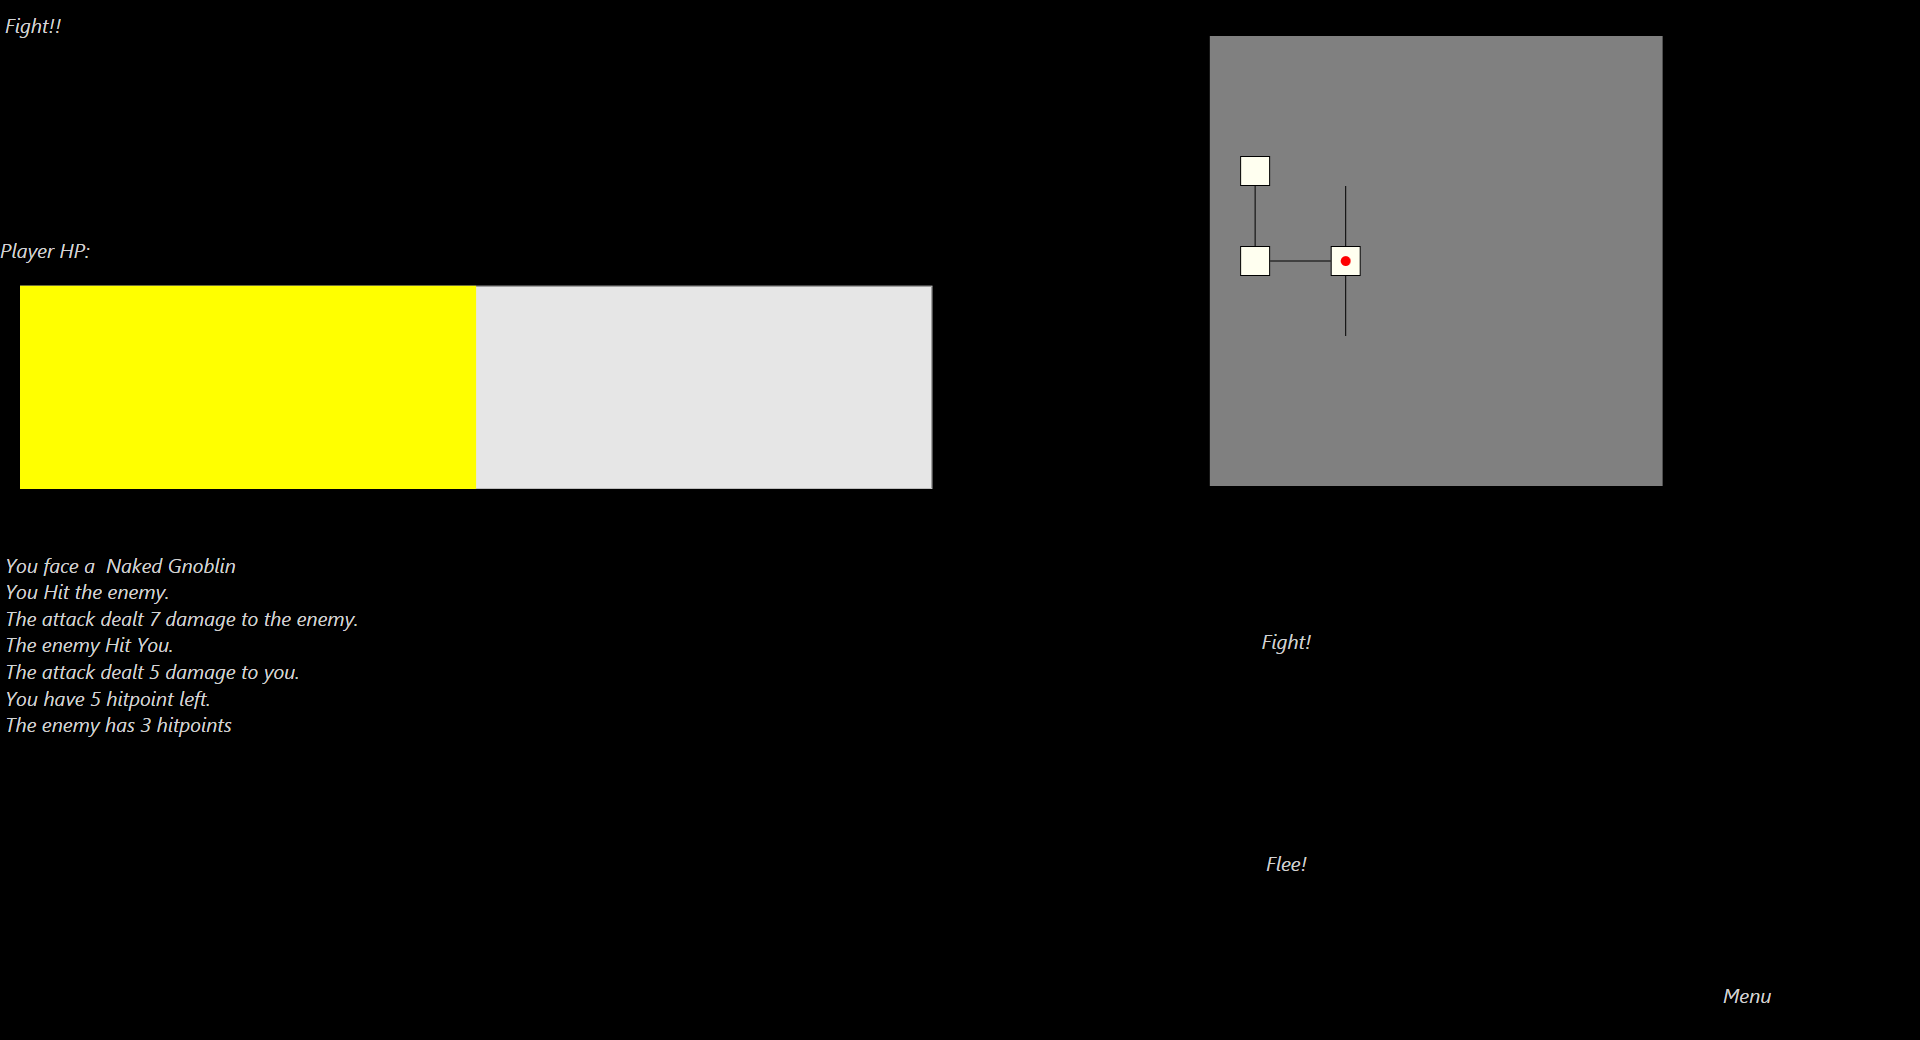
\includegraphics[width = \textwidth]{02-Body/Images/combat_final.PNG}
\caption{Combat view er baseret på room view. Her præsenters spilleren for info om en fjende og hvordan kampen mod fjenden går.}
\label{fig:Design-FE-impl-combat}
\end{figure}

\subsubsection{Settings view}

I settingsmenuen (\autoref{fig:Design-FE-impl-settings}) er det muligt at vælge lydstyrke for musikken i spillet (samt slukke helt for musikken) og vælge mellem tre skærmopløsninger (1280x720, 1920x1080 og 2k). Det tre valgmuligheder er valgt til at teksten på skærmen stadig er læselige. Kortet i Room og Combat view skalerer med skærmopløsningen, men sætter en nedre grænse på 300x300 pixel. Tekststørelsen gør dog at den praktiske nedre grænse, hvor spillet ser ud som det skal, er 1280x720. Ved skærm opløsning større end 2k bliver teksten og kortet for småt til at kunne ses ordentligt, hvorfor 2k er en naturlig øvre grænse for skærmopløsningen. Alle opløsninger imellem de to grænser burde være i orden (så længe det bare nogenlunde følger en 4:3 eller 16:9 ratio).\\

\noindent For at sørge for at den valgte skærmopløsning er brugt i alle views er der oprettet et objekt til at holde informationer om blandt andet indstillinger, samt andre informationer, som det ønskes at kunne tilgå fra flere forskellige views uden at være nødsaget til at sende data med rundt, når der skiftes mellem views. Dette objekt følger et singleton design pattern, og den samme instance af objektet kan derfor tilgås fra alle de view som skal bruge informationer derfra, på den måde opnås det at der kan sættes globale indstillinger som kan bruges på alle views uden at informationen skal sendes med i et skærmskift.\\

\noindent
Settings menuen kan tilgås fra både main menu og ingame menu, og det er derfor nødvendigt at spillet ved hvilken menu brugeren kommer fra, sådan at brugeren kan komme tilbage til den rigtige menu, når settings menuen forlades, ved at der trykkes på back-knappen. Til dette bruges singleton objektet fra tidligere afsnit også, da det gør det nemt at bringe informationen mellem views. Dette bruges også i ingame menu, da denne kan tilgås fra både room view og combat view og skal kunne returnere brugeren til det rigtige view, når brugeren vælger at starte spillet igen.

\begin{figure}[H]
\centering
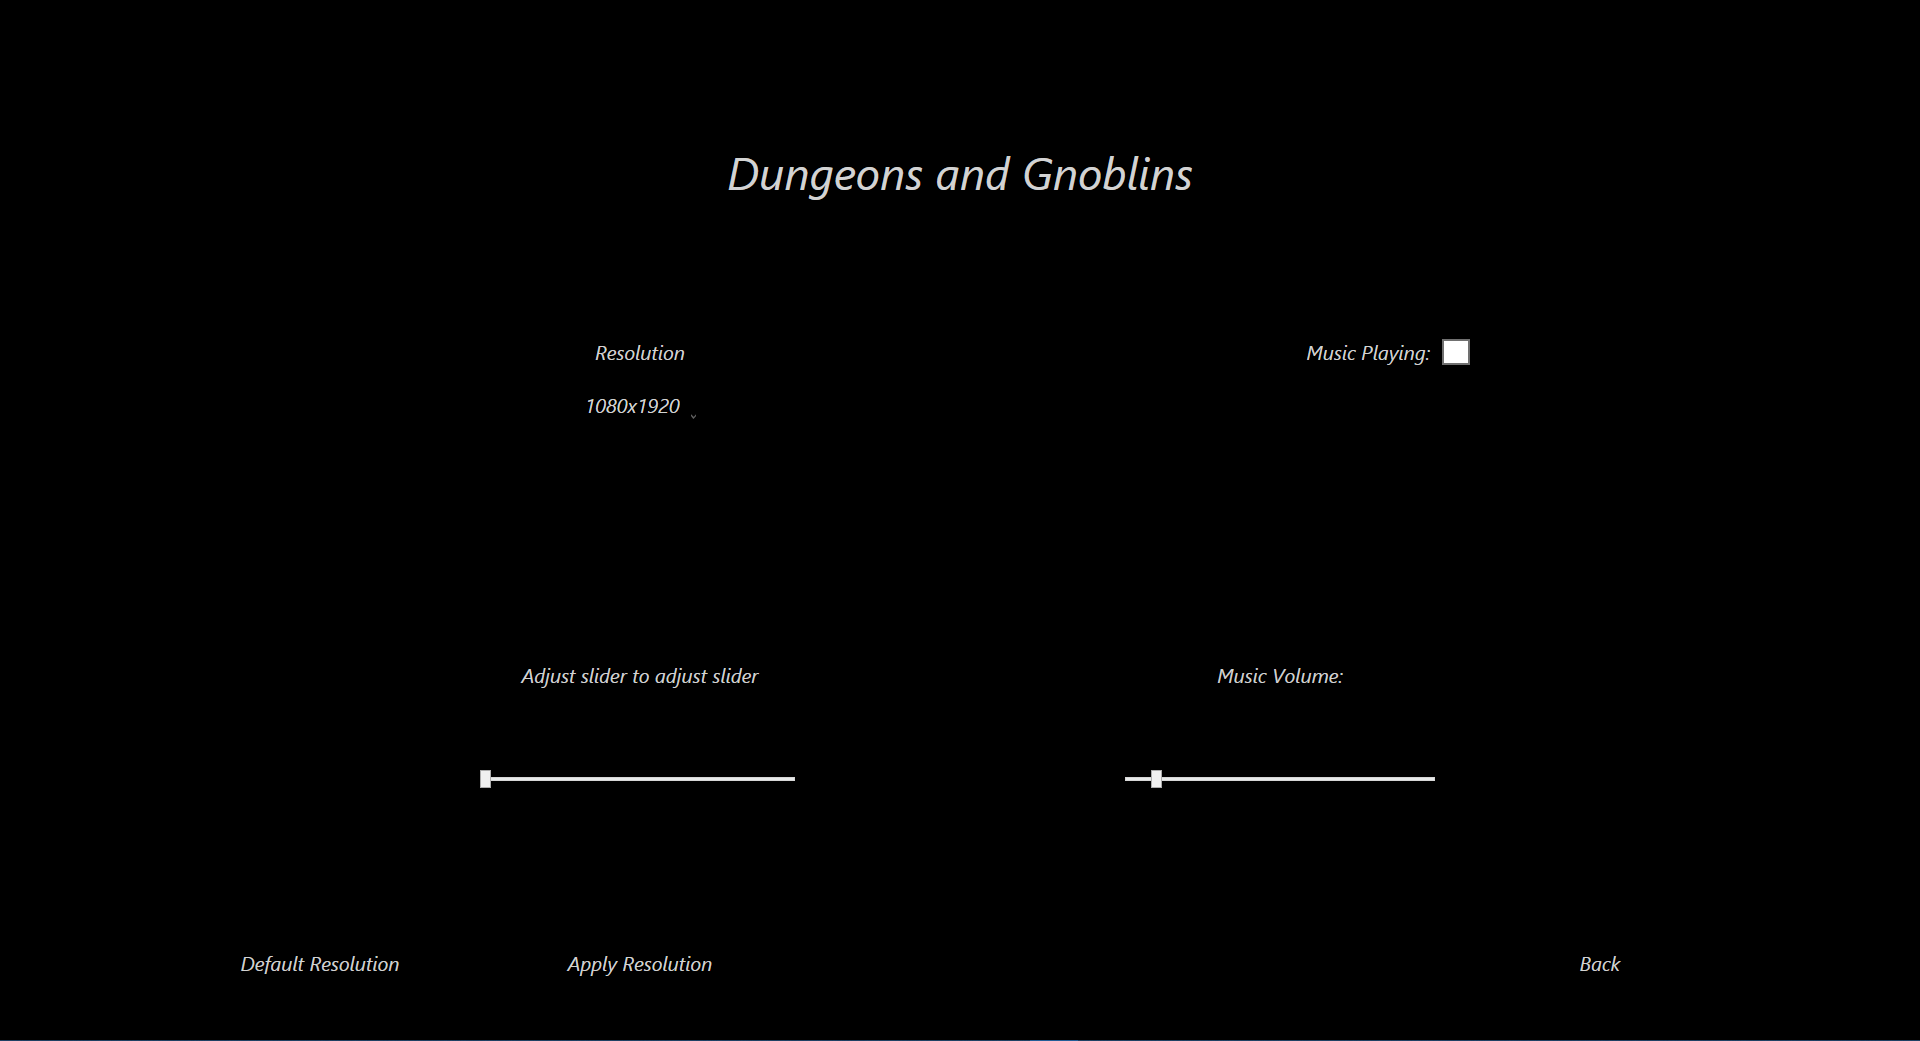
\includegraphics[width = \textwidth]{02-Body/Images/SettingsMenu_final.PNG}
\caption{Menu til at ændre spillets indstillinger. Det er her muligt at vælge skærmopløsning og lydstyrke, samt tænde og slukke for musikken. Back knappen fører tilbage til enten main menu eller ingame menu, afhængig af hvilke menu man tilgik settings menuen fra.}
\label{fig:Design-FE-impl-settings}
\end{figure}

\subsubsection{Load view}

Load (\autoref{fig:Design-FE-impl-load}) og Save menuerne præsenterer spilleren med en liste af gemte spil, som brugeren kan hente, eller gemme. Dette opnås ved at der hver gang spilleren åbner en af de to menuer, hentes en liste af tilgængelige 'save-games', som via databinding, præsenteres for brugeren. Når der trykkes på Save/Load sendes den fornødne kommando til backenden og backenden tager fat i databasen og udfører enten save eller load kommandoen.

\begin{figure}[H]
\centering
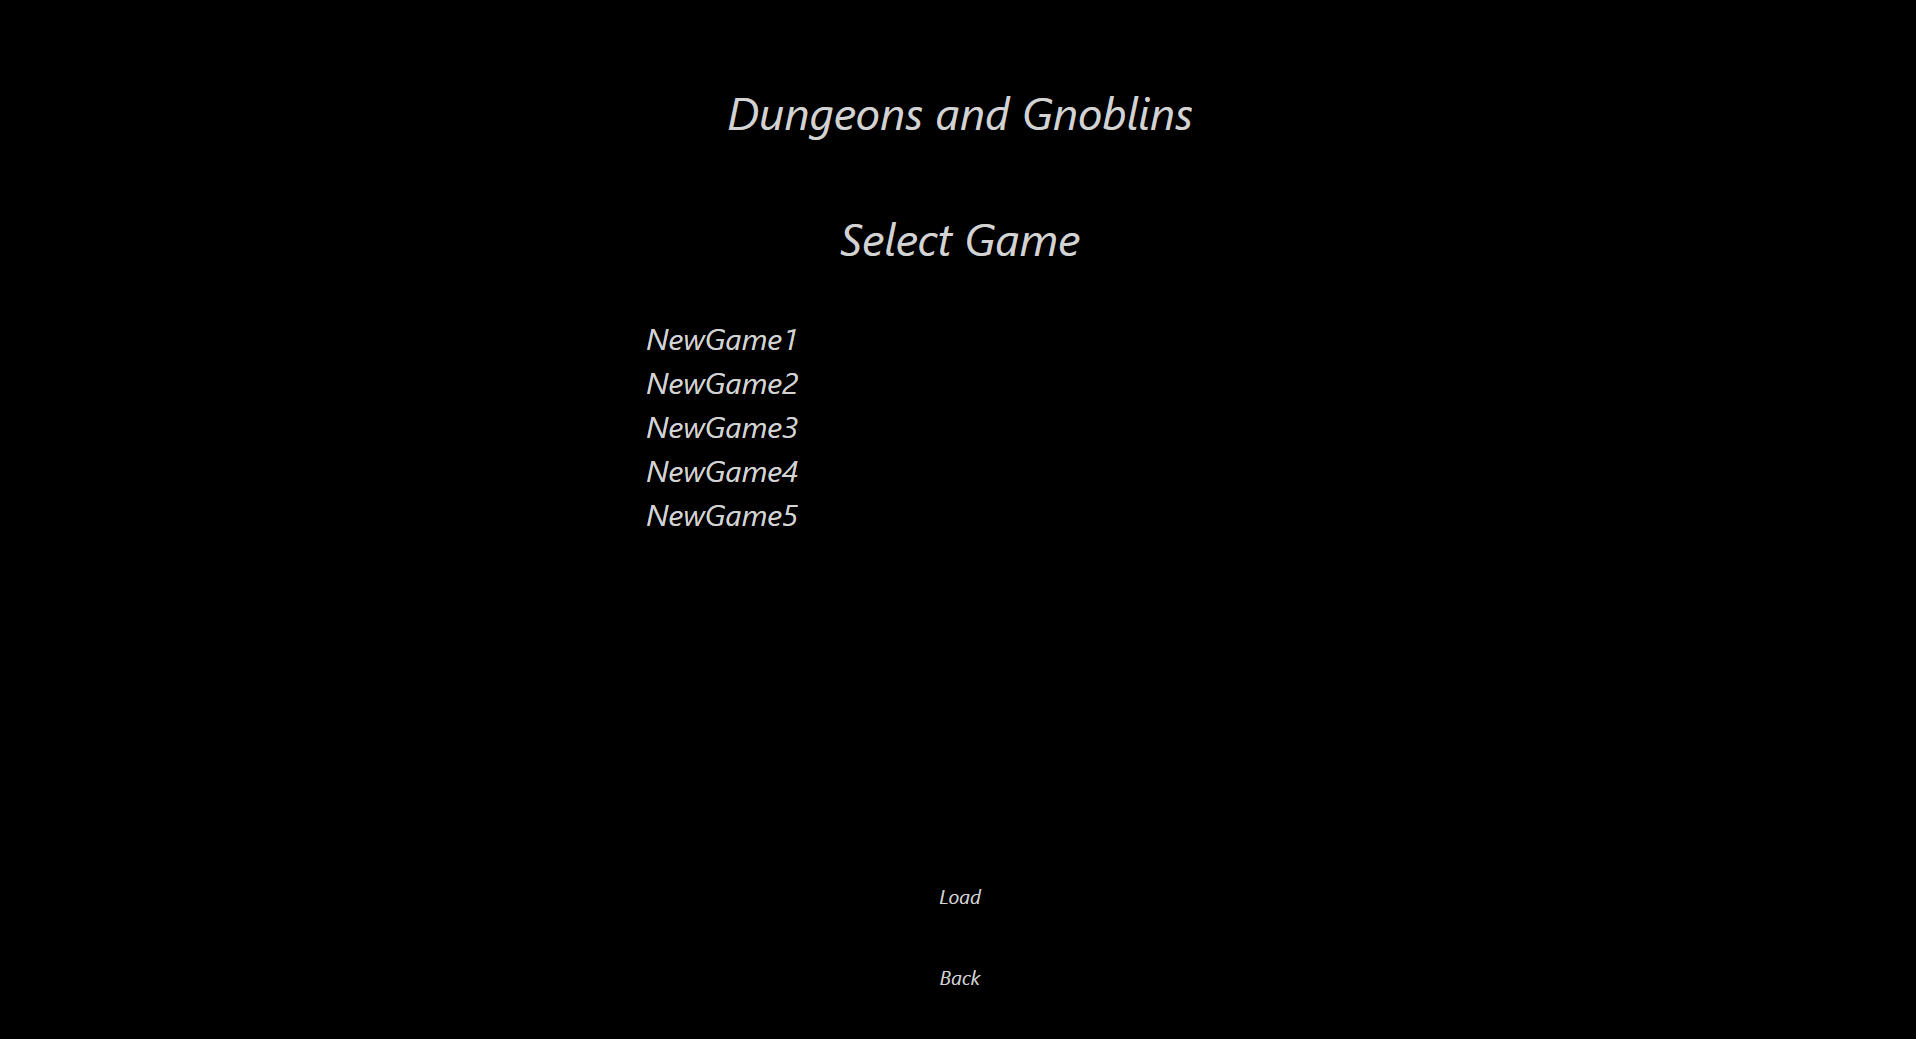
\includegraphics[width = \textwidth]{02-Body/Images/LoadMenu_final.png}
\caption{Load menu view. Her præsenteres spilleren for alle gemte spil. Disse hentes fra databasen hver gang spilleren går ind i load menuen.}
\label{fig:Design-FE-impl-load}
\end{figure}

\subsubsection{Note om Baggrundsfarver}
Da den generelle baggrundsfarve i spillet er sort er alle spillets interface elementer oprettet så baggrundsfarven matcher. Dette er for det meste nemt opnået ved brug af WPF styles, f.eks.:
\begin{lstlisting}
<Style x:Key="textBoxStyle" TargetType="TextBox">
    <Setter Property="Background" Value="{StaticResource backgroundColor}"/>
    <Setter Property="Foreground" Value="{StaticResource textColor}"/>
    <Setter Property="FontSize" Value="25"/>
    <Setter Property="FontStyle" Value="Italic"/>
    <Setter Property="BorderThickness" Value="1"/>
</Style>
\end{lstlisting}
men enkelte elementer (så som resolution dropdown menu, brugt i settings menuen) viste sig at være betydeligt mere omfattende. Det viser sig at det valgte element (WPF combobox) ikke tillader at baggrundsfarven for dropdown elementerne ændres i Windows 8 eller senere. Løsningen er at lave en kopi af hele templaten (ca. 300 linjer kode) for combobox og ændre 3-4 linjer. \cite{comboBox}

\newpage
